\documentclass[12pt, a4paper]{report}
\usepackage[utf8]{inputenc}
\newcommand\preamble{
    \usepackage[italian]{babel}
    \usepackage{geometry}
    \usepackage{amsmath}
    \usepackage{amssymb}
    \usepackage{graphicx}
    \usepackage[dvipsnames]{xcolor}
    \usepackage{ulem}
    \usepackage{listings}
    \usepackage{tikz}
    \usetikzlibrary{shapes.geometric, arrows}
    \usepackage{array}
    \usepackage{varwidth}
    
    \let\olditemize\itemize
    \renewcommand\itemize{\olditemize\setlength\itemsep{0em}}

    \tikzstyle{process} = [rectangle, minimum width=3cm, minimum height=1cm, text centered, text width=3cm, draw=black, fill=orange!30]
    \tikzstyle{decision} = [diamond, minimum width=3cm, minimum height=1cm, text centered, text width=2cm, draw=black, fill=green!30]
    \tikzstyle{arrow} = [thick,->,>=stealth]
    \geometry{left=1cm, right=1cm, top=2cm, bottom=2cm}
}
\newcommand{\customfbox}[1]{
    \begin{center}
        \fbox{\parbox{\dimexpr\linewidth-2\fboxsep-2\fboxrule\relax}{\centering #1}}
    \end{center}
}

% Definizione delle variabili
\newcommand{\imagePath}{Immagini/logoUni.png}

% Definizione del comando per la pagina di titolo con argomenti
\newcommand{\customTitlePage}[2]{
    \newcommand{\courseTitle}{#1}
    \newcommand{\academicYear}{#2}
    
    \begin{titlepage}
        \centering
        \includegraphics[width=0.5\textwidth]{\imagePath}\par\vspace{1cm}
        {\scshape\LARGE Università degli Studi di Genova \par}
        \vspace{1.5cm}
        {\huge\bfseries \courseTitle \par}
        \vspace{2cm}
        {\Large\itshape Lorenzo Vaccarecci \par}
        \vfill
        \academicYear
    \end{titlepage}
}


\preamble

\begin{document}
\customTitlePage{Fondamenti di Ingegneria del Software}{2024-2025}
\newpage
\tableofcontents
\chapter{Modelli di processo di sviluppo software}
\section{Introduzione}
\customfbox{\textbf{Processo}: insieme strutturato e organizzato di attività che si svolgono per ottenere un risultato.}
Perchè modellare il processo? Per dare ordine, controllo e ripetibilità con l'intenzione di migliorare la produttività e la qualità del prodotto.
\subsection{Processo prescrittivo e adattivo}
\begin{itemize}
    \item \textbf{Processo prescrittivo}: un processo che segue un modello predefinito e rigido, con passaggi specifici e ben definiti.
    \item \textbf{Processo adattivo}: un processo che permette modifiche e adattamenti durante il suo svolgimento.
\end{itemize}
Perchè studiare  i modelli di processo? Perchè uno dei compiti dei manager aziendali è quello di decidere il modello di processo da adottare considerando la tipologia del software da progettare e il personale disponibile.
\section{Modelli di processo}
\section{Code and Fix}
\begin{minipage}{0.4\textwidth}
\begin{itemize}
    \item Si arriva al codice finale "per tentativi"
    \item Non adatto per progetti grandi con tanti sviluppatori
    \item \textcolor{red}{Non è un modello di processo vero e proprio}
\end{itemize}
\end{minipage}
\hspace{0.05\textwidth}
\begin{minipage}{0.5\textwidth}
    \begin{tikzpicture}[node distance=2cm]
        \node (start) [process] {Capire i requisiti};
        \node (process1) [process, below of = start] {Codifica da zero, esecuzione e test};
        \node (dec1) [decision, below of = process1, yshift = -1cm] {Passano i test?};
        \node (process2a) [process, below of = dec1, yshift = -1cm] {Aggiustamento del codice, ri-esecuzione e test};
        \node (stop) [process, left of = dec1, xshift = -2cm] {Consegna del codice};
        \draw [arrow] (start) -- (process1);
        \draw [arrow] (process1) -- (dec1);
        \draw [arrow] (dec1) -- node[anchor=east] {no} (process2a);
        \draw [arrow] (dec1) -- node[anchor=south] {si} (stop);
        \draw [arrow] (process2a.east) -| ++(1,0) |- ([yshift=-0.3cm]process1.south); 
    \end{tikzpicture}
\end{minipage}
\section{Modello a cascata}
\begin{minipage}{0.5\textwidth}
\begin{itemize}
    \item \textcolor{red}{Storicamente il primo modello del processo di sviluppo software}
    \item Ogni fase produce un prodotto che è l'input della fase successiva
    \item Con il modello waterfall abbiamo il passaggio dalla dimensione artigianale alla produzione industriale del software
    \item Molto rigido: non si può tornare indietro
\end{itemize}
\end{minipage}
\hspace{0.05\textwidth}
\begin{minipage}{0.4\textwidth}
    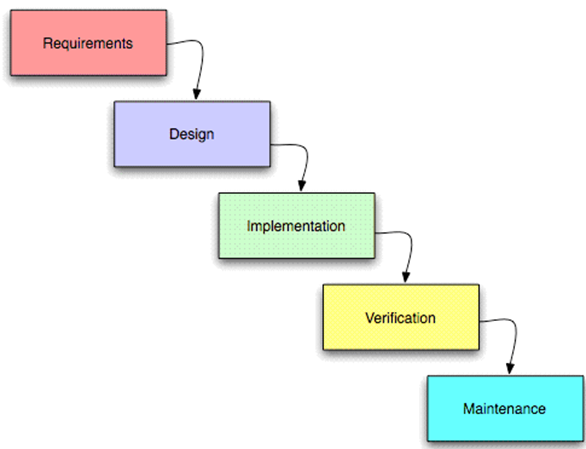
\includegraphics[width=\linewidth]{Immagini/waterfall.png}
\end{minipage}
\begin{center}

\begin{tabular}{|p{0.45\textwidth}|p{0.45\textwidth}|}
    \hline
    \textbf{\textcolor{green}{Vantaggi}} & \textbf{\textcolor{red}{Svantaggi}} \\
    \hline
    Enfasi su aspetti come l'analisi dei requisiti e il progetto di sistema trascurati nell'approccio code \& fix & Lineare, rigido, monolitico: no feedback tra fasi, no parallelismo, \textcolor{red}{unica data di consegna} \\
    \hline
    Pospone l'implementazione dopo avere capito i bisogni del cliente & La consegna avviene dopo anni, intanto i requisiti cambiano o si chiariscono: così viene consegnato software obsoleto \\
    \hline
    Introduce disciplina e pianificazione & Viene prodotta troppa documentazione poco chiara: l'utente spesso non conosce tutti i requisiti all'inizio dello sviluppo \\
    \hline
    E' applicabile se i requisiti sono chiari e stabili & Alcuni difetti superati da modello waterfall con feedback e iterazioni \\
    \hline
\end{tabular}
\end{center}
\subsection{Studio di fattibilità}
\begin{itemize}
    \item Fase che precede lo sviluppo vero e proprio
    \item Viene analizzata la fattiblità e convenienza del progetto
    \item Stima dei costi
    \item Si valuta il Return Of Investment (ROI)
\end{itemize}
\subsection{Varianti del modello a cascata}
\begin{itemize}
    \item Cascata con prototipazione: prima di iniziare lo sviluppo si costruisce un prototipo "usa e getta" con il solo scopo di fornire agli utenti una base concreta per meglio definire i requisiti.
    \item Cascata con feedback e iterazioni: posso tornare a una fase precedente. \begin{center}
        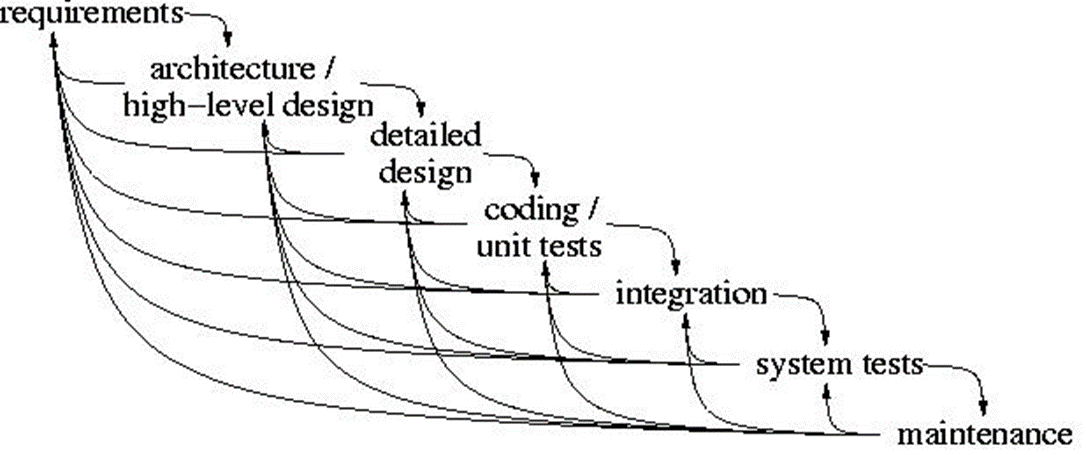
\includegraphics[width=0.8\linewidth]{Immagini/waterfallfeedback.png}
    \end{center}
    \item V-Model: \begin{itemize}
        \item Enfasi sulle fasi di testing
        \item Evidenzia come le attività di testing (parte destra della V) sono collegate a quelle di analisi e progettazione (parte sinistra della V)
        \item Ogni controllo fatto a destra che non dia buon esito porta a un rifacimento/modifica di quanto fatto a sinistra
        \item \textbf{Parallelismo}: creazione dei test e una volta che ho il codice li eseguo
        \item \textcolor{red}{Problemi (anche per Waterfall)}: \begin{itemize}
            \item Versione funzionante solo alla fine!
            \item Errore in fase iniziale può avere conseguenze disastrose
        \end{itemize}
    \end{itemize}
    \begin{center}
        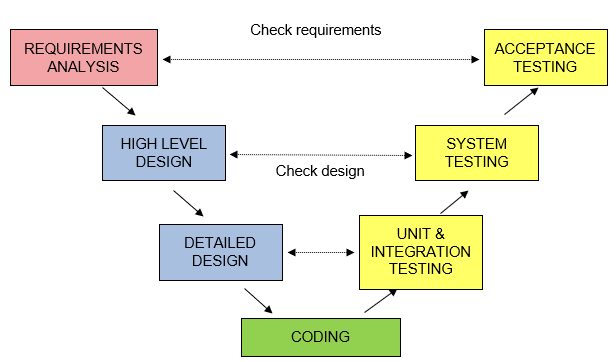
\includegraphics[width=0.5\linewidth]{Immagini/vmodel.png}
    \end{center}
\end{itemize}
\section{Modelli evolutivi}
\customfbox{Idea: sviluppare un implementazione iniziale, esporla agli utenti e raffinarla attraverso successivi rilasci del SW (release)}
Sottocategorie:
\begin{itemize}
    \item Prototyping
    \item Modelli incrementali
    \item Modelli iterativi
\end{itemize}
\subsection{Modelli a Prototyping}
\begin{itemize}
    \item Realizzazione di un prototipo funzionante del sistema, su cui validare i requisiti (o l'architettura)
    \item Il prototipo ha meno funzionalità ed è meno efficiente
\end{itemize}
\begin{center}
    \begin{tabular}{|p{0.45\textwidth}|p{0.45\textwidth}|}
        \hline
        \textbf{\textcolor{green}{Vantaggi}} & \textbf{\textcolor{red}{Svantaggi}} \\
        \hline
        Permette di raffinare requisiti definiti in termini di obiettivi generali e troppo vaghi & Il prototipo è un meccanismo per identificare i requisiti, spesso da "buttare": problema economico e psicologico, il rischio è di non farlo e così scelte non ideali diventano parte integrante del sistema \\
        \hline
        Rilevazione precoce di errori di interpretazione & \\
        \hline
    \end{tabular}
\end{center}
\subsection{Modelli Iterativi-Incrementali}
\begin{itemize}
    \item Sviluppo di varie release,  di cui solo l'ultima è completa
    \item Dopo la prima release, si procede in parallelo
    \item Le fasi di sviluppo vengono percorse più volte
\end{itemize}
\begin{center}
    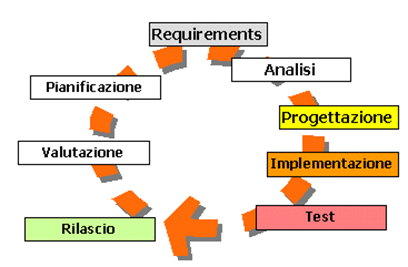
\includegraphics[width=0.5\linewidth]{Immagini/iterativoincrementale.png}
\end{center}
\subsubsection{Modelli Incrementali}
\begin{itemize}
    \item Ogni release aggiunge nuove funzionalità
    \item Nella fase di pianificazione si decide il requisito/funzionalità da includere nella release successiva.
    \item Si trattano per prime le funzionalità ad alto rischio
    \item Si cerca di massimizzare il valore per gli utenti
\end{itemize}
\subsubsection{Modelli Iterativi}
\begin{itemize}
    \item Da subito sono presenti tutte (o buona parte) delle funzionalità che sono via via raffinate, migliorate
\end{itemize}
\section{Modello a spirale}
\begin{itemize}
    \item Sistemi di grandi dimensioni
    \item Approccio "evolutivo" con interazioni continue fra cliente e developer
    \item Modello "risk-driver": tutte le scelte sono basate sui risultati dell'analisi dei rischi
    \item 'Meta-modello': dà un'idea generale ma quando si inizia a lavorare bisogna scegliere un modello esistente \begin{itemize}
        \item Requisiti chiari e stabili $\rightarrow$ modello a cascata
        \item Requisiti confusi $\rightarrow$ prototipo
    \end{itemize}
\end{itemize}
\customfbox{\textbf{Rischio}: circostanza potenzialmente avversa in grado di pregiudicare lo sviluppo e la qualità del software}
\textcolor{red}{Ogni scelta/decisione ha un rischio associato}, due caratteristiche importanti nella valutazione di un rischio sono: \begin{itemize}
    \item Gravità delle conseguenze
    \item Probabilità che si verifichi la circostanza
\end{itemize}
\begin{center}
    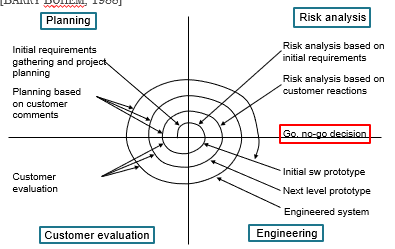
\includegraphics[width=0.7\linewidth]{Immagini/spirale.png}
\end{center}
\begin{itemize}
    \item \textbf{Planning}: determinazione di obbiettivi, alternative, vincoli
    \item \textbf{Risk Analysis}: analisi delle alternative e identificazione/risoluzione dei rischi
    \item \textbf{Engineering}: sviluppo del prodotto di successivo livello
    \item \textbf{Customer Evaluation}: valutazione dei risultati dell'engineering dal punto di vista del cliente
\end{itemize}
\begin{center}
    \begin{tabular}{|p{0.45\textwidth}|p{0.45\textwidth}|}
        \hline
        \textbf{\textcolor{green}{Vantaggi}} & \textbf{\textcolor{red}{Svantaggi}} \\
        \hline
        Adatto allo sviluppo di sistemi complessi & Non è un rimedio universale (panacea) \\
        \hline
        Primo approccio che considera il rischio (risk-driver) & Necessita competenze di alto livello per la stima dei rischi \\
        \hline
        & Richiede  un'opportuna personalizzazione ed esperienza di utilizzo \\
        \hline
        & Se un rischio rilevante non viene scoperto o tenuto a bada si inizia da zero \\
        \hline
    \end{tabular}
\end{center}
\section{Unified Process}
\begin{itemize}
    \item Specifico per sistemi ad oggetti, con uso di notazione UML per tutto il processo
    \item Guidato dagli \textbf{Use Case}
    \item Incorpora molte delle idee 'buone' dal modello a spirale
    \item Meta-modello
    \item Supportato da tool(visuali) in ogni fase
    \item Processo prescrittivo per eccellenza
\end{itemize}
\subsection{Le iterazioni}
\begin{itemize}
    \item Possibili diverse iterazioni che terminano con il rilascio del prodotto
    \item Ogni iterazione consiste di quattro fasi (anche ripetute più volte) che terminano con una milestone (= rilascio di artefatti soggetti a controllo)
    \item Ogni fase è costituita da diverse attività: \begin{itemize}
        \item Requisiti (R)
        \item Analisi (A)
        \item Design (D)
        \item Codifica (C)
        \item Testing (T)
    \end{itemize}
\end{itemize}
\subsection{Le fasi}
\begin{itemize}
    \item Inception: studio di fattibilità, requisiti essenziali del sistema, risk analysis
    \item Elaboration: sviluppa la comprensione del dominio e del problema, gli Use Case della release da rilasciare, l'architettura del sistema
    \item Construction: Design (in UML), codifica e testing del Sistema
    \item Transition: Messa in esercizio della release nel suo ambiente (deploy), training e testing da parte di utenti fidati
\end{itemize}
\section{Sviluppo basato sui componenti}
Modello che va nella direzione del \textbf{riutilizzo del software}
\begin{center}
    \begin{tabular}{|p{0.45\textwidth}|p{0.45\textwidth}|}
        \hline
        \textbf{\textcolor{green}{Vantaggi}} & \textbf{\textcolor{red}{Svantaggi}} \\
        \hline
        Riduce la quantità di software da scrivere & Sono necessari dei compromessi: requisiti iniziali potrebbero differire da quelli che si possono soddisfare con le componenti disponibili \\
        \hline
        Riduce i costi totali di sviluppo e i rischi & Integrazione non sempre facile \\
        \hline
        Consegne più veloci & Spesso i componenti usati sono fatti evolvere dalla ditta produttrice senza controllo di chi li usa \\
        \hline
    \end{tabular}
\end{center}
\section{Metodi Plan-Driven e Agili}
\begin{center}
    \begin{tabular}{|p{0.45\textwidth}|p{0.45\textwidth}|}
        \hline
        \textbf{Plan-Driven} & \textbf{Agile} \\
        \hline
        Seguono un approccio classico dell'ingegneria dei sistemi fondato su processi ben definiti e ocn passi standard & Rispondere ai cambiamenti dei requisiti in modo veloce \\
        \hline
        & Filosofia del programmare come "arte" piuttosto che processo industriale \\
        \hline
        & Cosa più importante soddisfare il cliente e non seguire un piano (contratto)\\
        \hline
    \end{tabular}
\end{center}
\begin{figure}[h]
    \centering
    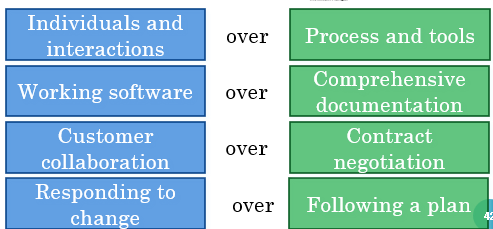
\includegraphics[width=0.5\linewidth]{Immagini/agilemanifesto.png}
    \caption{The Agile Manifesto}
\end{figure}
\subsection{Come scegliere?}
\textbf{Metodi plan-driven}: \begin{itemize}
    \item Sistemi grandi e comploessi, safety-critical o con forti richieste di affidabilità
    \item Requisiti stabili e ambiente predicibile
\end{itemize}
\textbf{Metodi agili}: \begin{itemize}
    \item Sistemi e team piccoli, clienti e utenti disponibili, ambiente e requisiti volatili
    \item Team con molta esperienza
    \item Tempi di consegna rapidi
\end{itemize}
\newpage
\section{DevOps}
Metodo di sviluppo evolutivo
\begin{figure}[h]
    \centering
    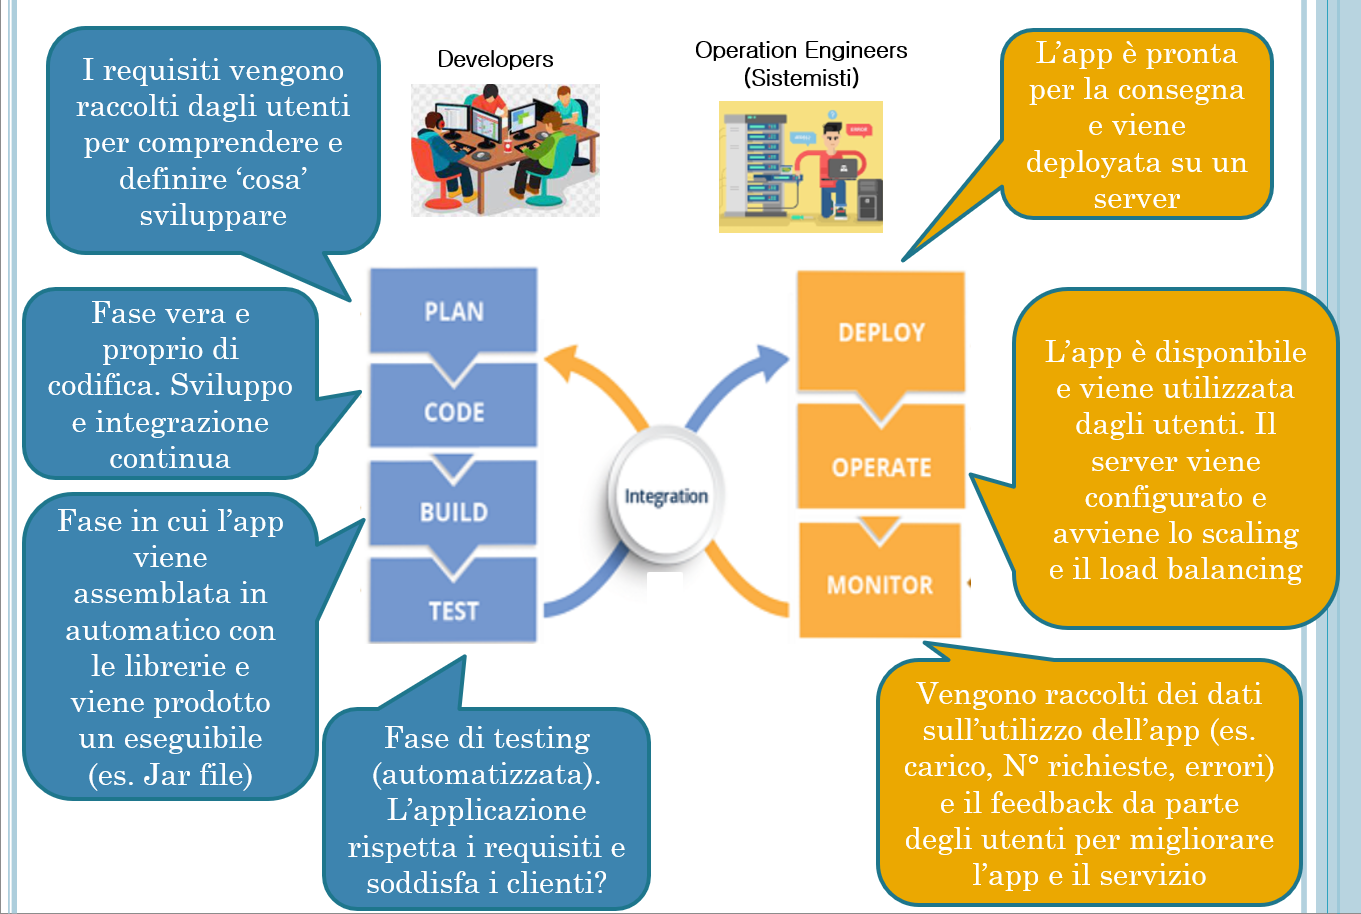
\includegraphics[width=0.8\linewidth]{Immagini/devops.png}
    \caption{DevOps}
\end{figure}
\subsection{Continuous Integration}
La Continuos Integration (CI), o Integrazione Continua, è una pratica di sviluppo software in cui i programmatori integrano frequentemente il proprio lavoro (codice) nel repository condiviso del progetto, in genere diverse volte al giorno.
\chapter{Ingegneria dei requisiti}
\section{Introduzione}
Descrivere 'qualcosa' che il sistema dovrà fare (una funzionalità) o un vincolo a cui deve sottostare
\begin{itemize}
    \item \textbf{Diversi livelli di astrazione}:\begin{itemize}
        \item Descrizione astratta ed imprecisa del sistema
        \item Descrizione dettagliata e matematica dello stesso
    \end{itemize}
\end{itemize}
\customfbox{Che cosa il sistema farà e non come!}
E' importante definire i requisiti in modo da evitare difetti in fasi avanzate del progetto, infatti i difetti dovrebbero essere scoperti il più presto possibile, ovvero a livello dei requisiti.
\section{Classificazione dei requisiti}
\begin{itemize}
    \item \textbf{Requisiti utente}: descrizione in linguaggio naturale delle funzionalità che il sistema dovrà fornire e dei vincoli operativi (\underline{sono scritti per (e con) il cliente})
    \item \textbf{Requisiti di sistema}: descrive in modo dettagliato le funzionalità che il sistema dovrà fornire (\underline{sono scritti per gli sviluppatori})
    \item \textbf{Requisiti funzionali}: descrivono ciò che il sistema dovrà fare, non come ma cosa
    \item \textbf{Requisiti non-funzionali}: definiscono vincoli sul sistema e sullo sviluppo del sistema, in generale riguardano la scelta di linguaggi, piattaaforme, strumenti, tecniche d'implementazione, ma anche: prestazioni, questioni etiche, ...
\end{itemize}
Un requisito etico può essere ad esempio che nella realizzazione dell'applicazione verranno utilizzato solo strumenti e servizi 'non proprietari' (es. no Microsoft)
\subsection{Esempio: Bancomat}
In \textcolor{red}{rosso} i requisiti funzionali, in \textcolor{blue}{blu} i requisiti non funzionali
\begin{itemize}
    \item \textcolor{red}{Il sistema deve mettere a disposizione le funzioni di prelievo, saldo e estratto conto}
    \item \textcolor{blue}{Il sistema deve essere disponibile a persone portatori di Handicap, deve garantire un tempo di risposta inferiore al minuto, e deve essere sviluppato su architettura X86 con sistema operativo compatibile con quello della Banca}
    \item \textcolor{red}{Le operazioni di prelievo devono richiedere autenticazione tramite un codice segreto memorizzato sulla carta}
    \item \textcolor{blue}{Il sistema deve essere facilmente espandibile, e adattabile alle future esigenze bancare}
\end{itemize}
\section{Requirements Engineering}
E' il termine usato per descrivere le attività necessarie per raccogliere, documentare e tenere aggiornato l'insieme dei requisiti di un sistema software.
\subsection{Scopo}
Lo scopo primario del RE è la produzione di un documento (il requirement document) che definisca le funzionalità e i servizi offerti dal sistema da realizzare (anche tenerlo aggiornato)
\subsection{Processo iterativo}
\begin{center}
    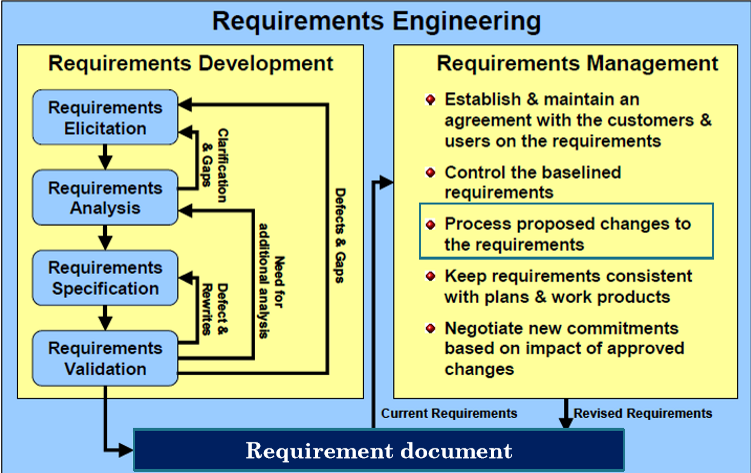
\includegraphics[width=0.6\textwidth]{Immagini/reiterativo.png}
\end{center}
\begin{itemize}
    \item \textbf{Elicitation}: \begin{itemize}
        \item Ottenere, estrarre, ricavare, tirar fuori i requisiti dal cliente e da altri partecipanti
        \item Il primo passo è identificare gli stakeholders\footnote{Stakeholder: persona veramente interessata allo sviluppo del progetto}
        \item Intervise, osservazioni sul luogo di lavoro, questionari, analisi dei prodotti dei competitors, workshop (brainstorming)
        \item Studio/analisi di leggi e regolamenti, help-desk reports, 'change requests' di prodotti analoghi, 'lessons learned' in progetti simili, ...
    \end{itemize}
    \item \textbf{Analisi dei requisiti}: \begin{itemize}
        \item I bisogni (user needs) degli stakeholders raccolti durante la fase di elicitation sono analizzati e raffinati
        \item Si cerca di capire se i requisiti sono corretti
        \item Si cercano di identificare i "missing requirements"
        \item Si identificano requisiti poco chiari
        \item Si risolvono i requisiti "contradditori o in conflitto"
        \item Viene stabilità la priorità (prioritizzazione): \begin{itemize}
            \item Per sapere cosa "tagliare" se non tutti potranno essere realizzati
            \item Scala numerica
            \item Scala MoSCoW: \begin{itemize}
                \item \textbf{Must have}: requisiti obbligatori
                \item \textbf{Should have}: requisiti importanti ma non indispensabili
                \item \textbf{Could have}: requisiti desiderabili ma non necessari
            \end{itemize} 
        \end{itemize}
    \end{itemize}
    \item \textbf{Definizione e specifica}: \begin{itemize}
        \item Definizione dei requisiti utente: costituisce un contratto fra le parti
        \item Specifica dei requisiti di sistema: costituisce "starting point" per la fase di design
    \end{itemize}
    \item \textbf{Validazione}: \begin{itemize}
        \item Esame della definizione/specifica dei requisiti per valutarne la qualità
        \item Di solito la convalida o validazione si effettua mediante 'formal peer reviewes'
        \item Scrivere dei casi di test a partire dai requisiti
        \item Sviluppare un prototipo
    \end{itemize}
    \item \textbf{Requirements Management}: \begin{itemize}
        \item Approvazione di alcune richieste di cambio dei requisiti
        \item Negoziazione con il cliente
        \item Impact analysis per i cambi richiesti
        \item Tenere allineati i requisiti e il codice (e casi di test)
        \item Tracciare il progresso di un progetto
    \end{itemize}
\end{itemize}
\section{Proprietà dei requisiti}
\begin{itemize}
    \item \textbf{Validità-correttezza}
    \item \textbf{Consistenza}: non ci sono requisiti contradditori
    \item \textbf{Completezza}: tutti gli aspetti che il cliente vuole sono coperti nei requisiti (in teoria)
    \item \textbf{Realismo}: non si chiede l'impossibile
    \item \textbf{Inequivocabilità (Unambiguos)}: ogni requisito dovrebbe avere solo un interpretazione
    \item \textbf{Verificabilità}: i requisiti vanno espressi in modo che siano testabili
    \item \textbf{Tracciabilità}: \begin{itemize}
        \item Ogni funzionalità implementata nel sistema deve poter essere fatta risalire a dei requisiti in modo semplice
        \item Ogni requisito nella requirement specification deve corrispondere ad uno nella requirement definition
    \end{itemize}
\end{itemize}
\section{Template/Schema dei requisiti}
Conviene attenersi a questo Schema
\begin{center}
    \large
    \texttt{<id>} il \texttt{<sistema>} deve \texttt{<funzione>}
\end{center}
Es. \texttt{R1.}Il sistema deve gestire tutti i regitratori di cassa del negozio (non più di 20)
\section{Analista software}
L'analista software o di sistema è la persona che:
\begin{itemize}
    \item si occupa dell'elicitazione dei requisiti
    \item analizza i requisiti
    \item scrive il documento dei requisiti (definizione e/o specifica)
    \item Comunica/spiega i requisiti a sviluppatori e altri stakeholder
\end{itemize}
Alcune competenze che un analista dovrebbe avere:
\begin{itemize}
    \item Arte della negoziazione
    \item Stabilire una strategia (problem solving)
    \item Giusta capacità di imporsi
    \item Ascoltare attentantemente
    \item Dono della sintesi
    \item Padronanza del linguaggio naturale
    \item Buona conoscenza del dominio (ad esempio in ambito medico o automobilistico)
\end{itemize}
\subsection{Consigli per un'intervista}
\begin{enumerate}
    \item Fare molte domande
    \item Ascoltare bene
    \item Mettere in discussione i quantificatori universali: 'tutto, ogni, sempre, ...'
    \item Annotare tutte le risposte
\end{enumerate}
\subsection{Importanza della comunicazione}
\begin{itemize}
    \item Elicitation = Attività molto delicata perchè mette in comunicazione due o più persone di realtà anche molto diverse
    \item Frequenti incomprensioni, che si ripercuotono sulla qualità dei requisiti
\end{itemize}
Occore fare molta attenzione a:
\begin{itemize}
    \item Diversità di significato che si attribuisce ai termini $\rightarrow$ possibile soluzione definizione del glossario: \begin{itemize}
        \item Per la spiegazione dei termini tecnici
        \item Per ridurre l'ambiguità dei termini usati
        \item Per "espandere" gli acronimi
    \end{itemize}
    \item Assunzioni nascoste (Hidden assumptions)
    \item Verbosità (= sovrabbondanza di parole)
    \item Mancanza di chiarezza/precisione
\end{itemize}
\section{Consigli finali}
\begin{itemize}
    \item Riuso di (parte di) requisiti
    \item Utilizzo di un glossario comune tra clienti, utenti e analisti
    \item Utilizzo di un 'buon' template/form
    \item Utilizzo di un software per la geitone/raccolta e analisi dei requisiti
\end{itemize}
\chapter{Definizione dei requisiti basata su use case}
\section{Cosa sono/servono}
\begin{itemize}
    \item Esprimere requisiti funzionali di un sistema
    \item Descrivere dal punto di vista di chi lo usa un sistema, il sistema è visto come una black-box
    \item Totalemnte indipendendti dal mondo OO
    \item Solo testo, formattato in modo standard (template)
    \item Visuale lo Use Case Diagram (UML)
    \item Gli use case esprimono l'interazione tra le entità (attori) che interagiscono con il sistema stesso
\end{itemize}
\section{Differenza tra requisito e use case}
\begin{itemize}
    \item \textbf{Requisito}: descrive una funzionalità dal punto di vista del sistema
    \item \textbf{Caso d'uso}: descrive una modalità di utilizzo del sistema da parte di un utilizzatore (punto di vista dall'utente)
\end{itemize}
La differenza sostanziale è nel modo in cui è presentata l'informazione
\section{Definizione dei requisiti basata su use case}
\begin{itemize}
    \item \textbf{Attore}: rappresenta un ruolo che un entità esterna "recita" interagendo con il sistema, da non confondere un ruolo con la cosa stessa \begin{itemize}
        \item \textbf{Primari}: chi guadagna qualcosa dal sistema (ad esempio un cliente Amazon)
        \item \textbf{Secondari}: chi produce qualcosa (o offre un servizio) per il sistema (ad esempio Paypal)
    \end{itemize}
    \item \textbf{Use case}: quello che gli attori 'possono fare' con il sistema
    \item \textbf{Relazioni}: tra gli attori e gli use case
    \item \textbf{Confini del sistema}: un rettangolo disegnato intorno agli use case per indicare i confini del sistema, quando si vuole costruire un sistema è la prima cosa da fare
\end{itemize}
\section{Scenario}
\customfbox{Uno scenario è una sequenza ordinata di interazioni tra un sistema e gli attori}
Rappresenta una particolare esecuzione di uno use case (istanza), e rappresenta un singolo cammino dello use case, sono usati per il testing. Si possono avere diversi scenari, ma in tutti l'attore può avere lo stesso scopo.
\section{Use Case}
\customfbox{Insieme di scenari che hanno in comune lo scopo finale dell'attore}
\begin{itemize}
    \item Gli use case in genere sono dati come testo strutturato
    \item I passi di uno use case sono testo facile da capire
    \item Viene usato il vocabolario del dominio dell'applicazione
    \item Gli use case sono descrizioni chiare, precide, generali e indipendenti dalle tecnologie
\end{itemize}
\subsection{Descrivere uno use case}
\begin{itemize}
    \item \textbf{Scenario principale}: scenario del mondo perfetto
    \item \textbf{Scenari secondari}: cosa può succedere di sbagliato o differente e come gestirlo
\end{itemize}
\subsection{Template}
\begin{itemize}
    \item \textbf{Nome dello use case}: è il goal dello use case \texttt{"breve frase verbale attiva"} in UpperCamelCase
    \item \textbf{Identificatore}: di solito numerico progressivo
    \item \textbf{Breve descrizione}: un paragrafo che fissa l'obbiettivo dello use case
    \item \textbf{Attori primari}: l'attore/gli attori primari dello use case
    \item \textbf{Attori secondari}: gli attori che "servono" per svolgere lo use case
    \item \textbf{Precondizioni}: vincoli sullo stato corrente del sistema
    \item \textbf{Scenario principale}: i passi che costituiscono lo use case
    \item \textbf{Postcondizioni}: condizioni che devono essere vere quando lo use case termina con successo l'esecuzione dello scenario principale
    \item \textbf{Scenari alternativi}: un elenco di alternative allo scenario principale
\end{itemize}
Uno scenario è costituito da un elenco di passi che devono essere concisi, numerati e ordinati temporalmente: \texttt{<numero> Il <Sistema/Attore> <qualche azione>}. Si ha una deviazione tutte le volte che 'ci si allontana' dallo scenario principale: \begin{itemize}
    \item \textbf{Semplici}: usare parola chiave \texttt{se} nella sequenza principale
    \item \textbf{Complesse}: scrivere sequenze degli eventi alternative che rappresentano errori o casi particolari che non ritornano sullo scenario principale
\end{itemize}
Si possono usare ripetizioni all'interno di una sequenza: \texttt{per} e \texttt{fintantochè}.\\
E' possibile che una sequenza venga attivata in qualunque momento della sequenza principale.
\section{Gerarchia attori}
\begin{center}
    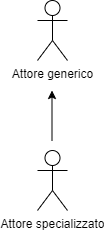
\includegraphics[width=0.2\textwidth]{Immagini/attori.png}
\end{center}
Come per le classi di Java, l'attore specializzato eredita le relazioni dell'attore generale
\section{Relazioni tra use case}
\begin{itemize}
    \item \textbf{Inclusione \texttt{<<include>>}}: \begin{itemize}
        \item Assomiglia al concetto di procedura/funzione
        \item Lo use case "principale" esegue i passi fino al punto di inclusione e passa il controllo allo use case incluso, alla fine il controllo ritorna allo use case principale
        \item Lo use case principale senza use case incluso risulta incompleto
    \end{itemize}
    \item \textbf{Estensione \texttt{<<extend>>}}: per estendere il comportamento di uno use case con un comportamento aggiuntivo (opzionale) rispetto allo use case base
    \item \textbf{Generalizzazione/specializzazione}: gli use case specializzati (figli) rappresentano delle varianti più specifiche dello use case generalizzato (genitore) da cui ereditano, i 'figli' possono \begin{itemize}
        \item Ereditare i passi del genitore
        \item Aggiungere nuovi passi
        \item Ridefinire (modificare) i pasi ereditati
    \end{itemize}
\end{itemize}
\chapter{Design architetturale}
\section{Introduzione}
\customfbox{Trasforma un problem in una soluzione (come)}
Il design definisce la struttura della soluzione invece l'implementazione la realizza, rendendola usabile.
\begin{itemize}
    \item \textbf{Architectural design (high-level)}: mappa i requisiti su architettura SW e componenti/sottosistemi
    \item \textbf{Component design (low-level)}: fissa dettagli dei componenti, specificando maggiormente la soluzione
\end{itemize}
Scelte tecnologiche:
\begin{itemize}
    \item \textbf{platform-independent design}: come pro ha il riuso
    \item \textbf{platform-specific design}: come pro aiuta i programmatori, per specifico si intende ad esempio nominare già le strutture dati specifiche per un linguaggio.
\end{itemize}
\subsection{Livelli di ri-uso}
\begin{itemize}
    \item \textbf{Clonazione}: si riutilizza interamente design/codice, con piccoli aggiustamenti
    \item \textbf{Design pattern}: buona soluzione a problema ricorrente
    \item \textbf{Stili architetturali}: architettura generica che suggerisce come decomporre il sistema
    \item \textbf{Software Frameworks}: insieme di classi e interfacce cooperanti che realizzano un design per uno specifico dominio applicativo o tipologia di app
\end{itemize}
\section{Design architetturale}
Processo di design per identificare:
\begin{itemize}
    \item le macro componenti di un sistema
    \item come avviene il controllo e la comunicazione tra componenti
\end{itemize}
Produce una descrizione dell'architettura software.
\section{Componenti}
\customfbox{Un modulo è un'unità del sistema che offre servizi ad altre unità, ma che non può essere considerato un sistema a se stante}
Un sottosistema è un sistema di per sè: può essere eseguito ed utilizzato anche "da solo". Di solito i sottosistemi sono composti da moduli ed hanno interfacce ben definite, che sono utilizzate per la comunicazione con altri sottosistemi.
\section{Diagramma a blocchi}
Un architettura software è normalmente espressa mediante un diagramma a blocchi che presenta un "overview" della struttura del sistema. I blocchi sono i componenti, i connettori rappresentano le "relazioni" tra i componenti.
\begin{center}
    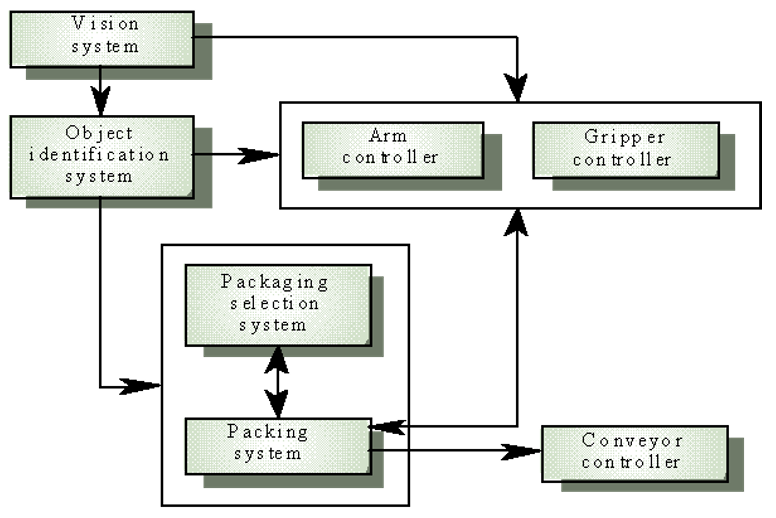
\includegraphics[width=0.5\textwidth]{Immagini/diagrammablocchi.png}
\end{center}
\section{Architettura SW}
\subsection{Proprietà del sistema}
\begin{itemize}
    \item \textbf{Performance}: tempi di risposta rapidi
    \item \textbf{Security}: difficile da "manomettere", dati sensibili protetti
    \item \textbf{Safety}: non creare "disastri"
    \item \textbf{Availability}: 24//7/365
    \item \textbf{Maintainability}: semplice da mantenere/evolvere
\end{itemize} 
\subsection{Vantaggi}
\begin{itemize}
    \item Guida lo sviluppo ed aiuta nella comprensione del sistema
    \item Documenta il sistema
    \item Aiuta a ragionare sull'evoluzione del sistema
    \item Supporta decisioni manageriali
    \item Facilita l'analisi di alcune proprietà
    \item Permette il riuso (Large-scale)
\end{itemize}
\subsection{Stili architetturali}
L'architettura di un sistema può conformarsi a uno stile architetturale
\begin{itemize}
    \item \textbf{Modello generico}: con caratteristiche specifiche che può essere istanziato/personalizzato
    \item \textbf{Layered}
    \item \textbf{Repository}
    \item \textbf{Client/server}
    \item \textbf{P2P}
    \item \textbf{Broadcast model}
    \item \textbf{Service Oriented Architecture}
    \item \textbf{Microservice}
\end{itemize}
Uno stile \textbf{strutturale} fornisce solo informazioni strutturali, uno \textbf{di controllo} anche informazioni (o solo) di controllo.\\
\customfbox{Conoscere gli stili architetturali può semplificare il problema di definire l'architettura software}
La maggioranze dei grandi sistemi sono \underline{eterogenei} e non seguono un singolo stile architetturale
\subsubsection{Elementi}
\begin{itemize}
    \item \textbf{Componenti}
    \item \textbf{Connettori}
\end{itemize}
\subsection{Layered}
\begin{itemize}
    \item Organizza il sistema in un insieme di livelli ognuno dei quali fornisce un insieme di servizi
    \item Un livello usa solo i servizi del livello inferiore
\end{itemize}
\begin{center}
    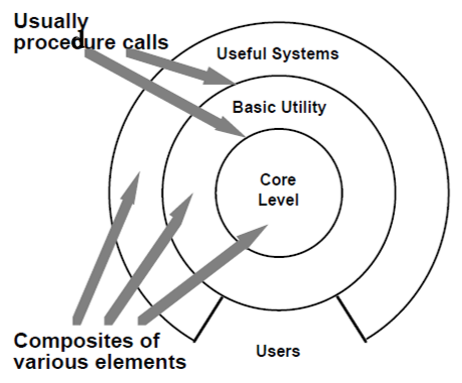
\includegraphics[width=0.4\textwidth]{Immagini/layered.png}
\end{center}
\subsection{Repository}
I dati condivisi sono mantenuti in un database centrale (repository o blackboard) a cui hanno accesso tutti i sotto-sistemi
\begin{center}
    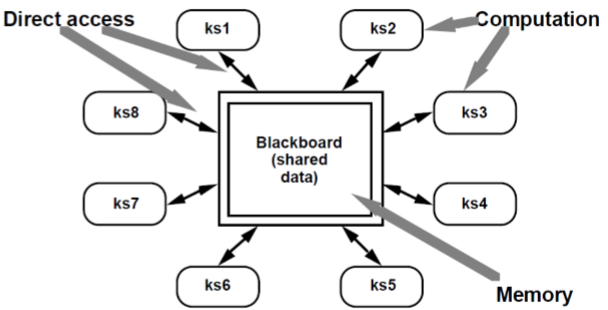
\includegraphics[width=0.5\textwidth]{Immagini/repository.png}
\end{center}
\subsection{Client/server}
\begin{itemize}
    \item Modello di sistema distribuito che mostra come i dati e la computazione possono essere distribuiti su: \begin{itemize}
        \item Insieme di server che forniscono servizi specifici
        \item Insieme di client che utilizzato tali servizi
    \end{itemize}
    \item Esiste una rete che permette ai client di accedere ai server
\end{itemize}
\subsubsection{Two-Tier}
Tre strati/componenti software:
\begin{itemize}
    \item Interfaccia utente (presentation logic)
    \item Gestione dei processi e logica (business o appl. logic)
    \item Gestione del DB (data logic)
\end{itemize}
Distribuiti in due livelli ($n$ client + $m$ server)
\begin{itemize}
    \item Client
    \item Server
\end{itemize}
\begin{center}
    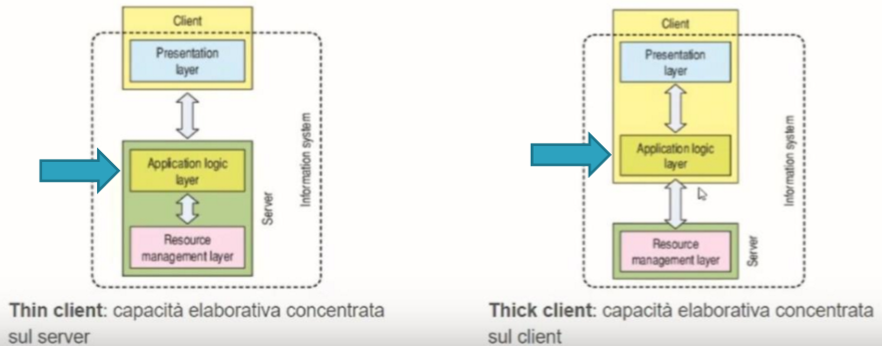
\includegraphics[width=0.8\textwidth]{Immagini/thinclientfatclient.png}
\end{center}
\subsubsection{Three-Tier}
\begin{itemize}
    \item Sul client resta solo l'interfaccia utente
    \item La logica del sistema risiede sull'Application server e gestisce multi-utenti
    \item Gli strati di logica e gestione DB sono distribuiti su più DB server
\end{itemize}
\subsection{Pipe and Filter}
\begin{itemize}
    \item I filtri effettuano trasformazioni che elaborano i loro input per produrre output
    \item Le pipe sono connettori che trasmettono i dati tra filtro e filtro
\end{itemize}
Ad esempio \texttt{ls -l | grep "Aug} dove l'output di \texttt{ls -l} viene passato a \texttt{grep "Aug"} grazie alla pipe
\subsection{Architetture eterogenee}
Ci sono due modi di combinare gli stili ottenendo così un architettura eterogenea:
\begin{itemize}
    \item Modo gerarchico
    \item Permettendo che una componente sia un mix di architetture
\end{itemize}
\subsection{Microservices}
\customfbox{Avere servizi separati e quindi potenzialmente più piccoli e facili da gestire (sviluppare, testare, deployare), anche dislocati su server diversi}
\subsubsection{Perchè?}
Se la app cresce:
\begin{itemize}
    \item La complessità aumenta
    \item Difficile trovare e risolvere bug
    \item Difficile effettuare  modifiche
    \item Tempi estesi per il deploy
    \item Complesso lavorare in parallelo (team)
\end{itemize}
\begin{center}
    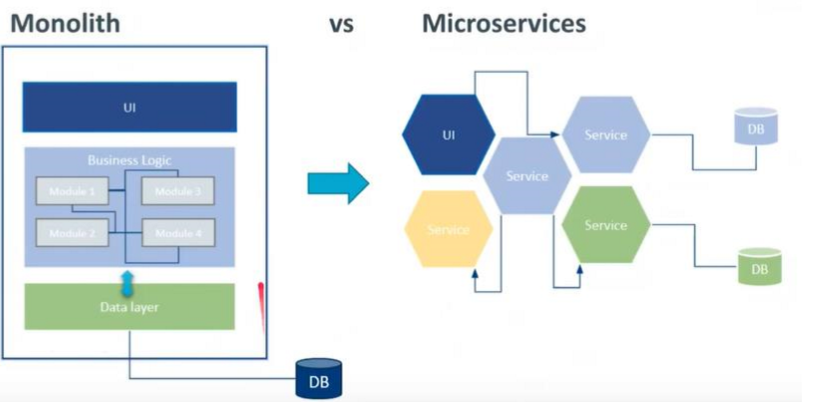
\includegraphics[width=0.8\textwidth]{Immagini/monolithvsmicroservice.png}
\end{center}
Ogni microservizio può essere scritto in un linguaggio di programmazione diverso ed avere diversi DBMS.
\subsubsection{Comunicazione}
\begin{itemize}
    \item \textbf{API Gateway}: espone un'interfaccia verso i client
    \item \textbf{REST}: le applicazioni basate su REST utilizzano le richieste HTTP per tutte e quattro le operazioni di \texttt{CRUD} (Create, Read, Update, Delete)
\end{itemize}
\subsubsection{Problemi}
\begin{itemize}
    \item Stabilire la dimensione dei micro servizi
    \item Sviluppo del meccanismo di comunicazione tra i servizi
    \item Esposizione ai disservizi di rete
    \item Gestione dello schema partizionato dei DB
    \item Difficoltà di testing
    \item Maggior consumo di risorse e memoria
\end{itemize}
\chapter{Design delle componenti}
\section{Fasi}
\begin{center}
    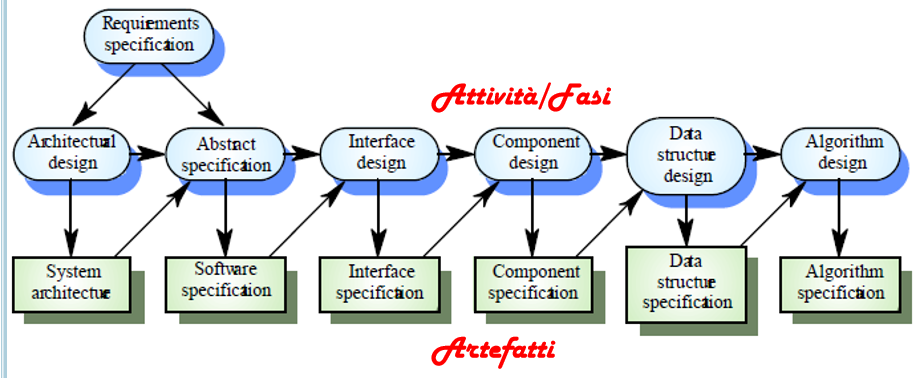
\includegraphics[width=0.7\textwidth]{Immagini/processocomponentifasi.png}
\end{center}
\section{Design by contract}
E' un metodo di design per il software che ha come obiettivo quello  di migliorarne la qualità e prescrive che il progettista debba definire specifiche precise delle interfacce dei classi/componenti software, basandosi sulla metafora di un contratto legale (il "contratto", viene creato per ogni componente del sistema \underline{prima che sia codificato}). L'idea centrale è che una componente software ha degli obblighi nei confronti delle altre componenti.
\subsection{Elementi di un contratto}
\begin{itemize}
    \item \textbf{Pre-condizione}: espressione a valori booleani rappresentante le aspettative sullo 'stato del mondo' prima che venga eseguita un'operazione
    \item \textbf{Post-condizione}: espressione a valori booleani riguardante lo 'stato del mondo' dopo l'esecuzione di un'operazione
    \item \textbf{Invariante di classe}: condizione che ogni oggetto della classe deve soddisfare quando è 'in equilibrio'
\end{itemize}
\textbf{Le precondizioni sono utili?} a prima vista potrebbe risultare inutile in quanto si possono aggiungere controlli all'interno del codice però chi è responsabile di questi controlli? Senza una dichiarazione esplicita  potremmo avere \begin{enumerate}
    \item \textbf{Troppi pochi controlli}
    \item \textbf{Troppi controlli}
\end{enumerate}
\subsection{Vantaggi}
\begin{itemize}
    \item Codifica: guida per lo sviluppatore durante la fase di codifica
    \item Migliorano la qualità del software: definisce quale componente è responsabile ad effettuare i controlli. Aiuta a scrivere operazioni semplici  che soddisfino un contratto ben definito
    \item Documentazione: \texttt{Pre}, \texttt{Post} e \texttt{Invarianti} documentano in  modo preciso cosa fa una componente/classe
    \item Testing: guida alla generazione di casi di test "black-box"
    \item Debugging: permette di trovare il "colpevole" di un malfunzionamento: \begin{itemize}
        \item Le eccezioni si sollevano quando il contratto è violato
    \end{itemize}
\end{itemize}
\section{Progettazione degli algoritmi}
E' l'attività più vicina alla codifica (spesso viene lasciata in parte o totalmente agli sviluppatori) e, di solito, si seguono i seguenti passi:
\begin{enumerate}
    \item Si analizza la descrizione di design della classe "target"
    \item Se esistono una o più operazioni che necessitano di un algoritmo, se  è possibile selezionare un algoritmo noto si seleziona altrimenti occorre definire un algoritmo e si sceglie una notazione e si progetta utilizzando la nozione di "stepwise refinement"
    \item Si usano i metodi formali per provare la correttezza dell'algoritmo proposto
\end{enumerate}
\begin{figure}[h]
    \centering
    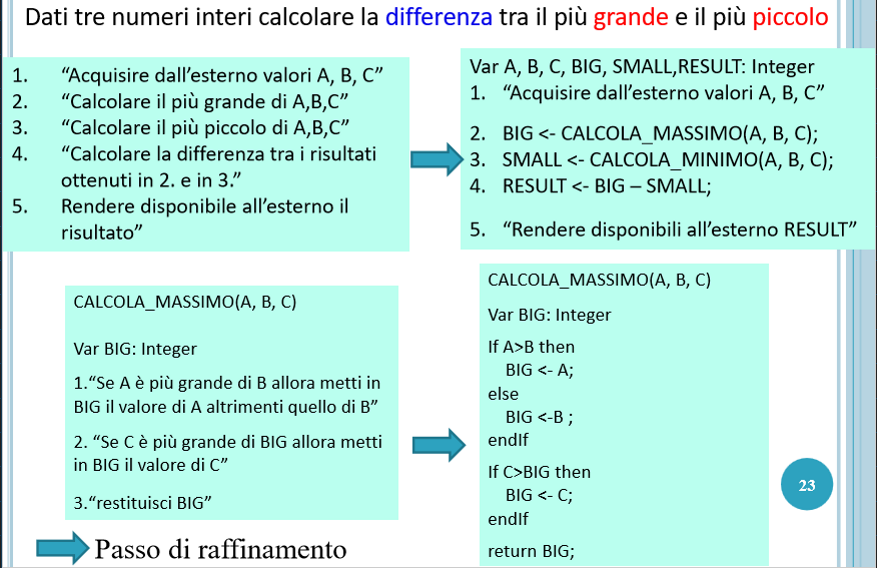
\includegraphics[width=0.6\textwidth]{Immagini/stepwiserefinement.png}
    \caption{Stepwise Refinement}
\end{figure}
\subsection{Notazioni}
Esistono diverse notazioni utilizzate per rappresentare un algoritmo:
\begin{itemize}
    \item \textbf{Visuali}: Activity Diagram di UML, Flowchart, Box Diagram, Structured Chart, Decision Table, \ldots
    \item \textbf{Testuali}:  Program Design Language (PDL) o pseudocodice
\end{itemize}
\subsubsection{PDL}
Il \textbf{Program Design Language} (PDL) o pseudocodice è un linguaggio semplificato che usa il vocabolario di un linguaggio naturale e la sintassi di un linguaggio di programmazione.
\section{Principi di progettazione}
\customfbox{I principi di progettazione guidano verso il raggiungimento degli obiettivi di qualità per il progetto}
Porta a produrre software: manutenibile, comprensibile, semplice da testare, riusabile, riparabile e portatile \ldots\\
Si possono applicare per tutti i sistemi non solo Object Oriented!
\subsection{Principi}
\subsubsection{Astrazione}
Permette di concentrarsi su un problema ad un determinato livello di astrazione, senza perdersi in dettagli irrilevanti. Nasconde informazioni che a un determinato livello non servono.\\
Forme di astrazione:
\begin{itemize}
    \item \textbf{Funzionale}:: definizione di una funzionalità indipendentemente dall'algoritmo che la implementa
    \item \textbf{di Dati}: definizione di un tipo di dato in base alle operazioni che su di esso possono essere fatte, senza definirne una struttura concreta
    \item \textbf{di Controllo}: definizione di un meccanismo di controllo senza indicarne i dettagli interni
\end{itemize}
\subsubsection{Decomposizione}
Cercare di risolvere un problema in una volta sola è in genere più difficile che risolverlo per parti.
\customfbox{\textbf{Legenda:} \begin{itemize}
    \item $P$ problema
    \item $C(P)$ complessità di $P$
    \item $E(P)$ effort (sforzo) per la risoluzione (software) di $P$
\end{itemize}}
Dati due problemi $P_{1}$ e $P_{2}$
\begin{itemize}
    \item Se $C(P_{1})>C(P_{2})$ allora vale $E(P_{1})>E(P_{2})$
    \item $C(P_{1}+P_{2})>C(P_{1})+C(P_{2})$ vale empiricamente
    \item $E(P_{1}+P_{2})>E(P_{1})+E(P_{2})$
\end{itemize}
L'ultima disequazione porterebbe a una conclusione sbagliata che se noi dividessimo il problema e quindi il software infinite volte l'effort di sviluppo diventerebbe nullo. In realtà entrano in gioco altre variabili:
\begin{center}
    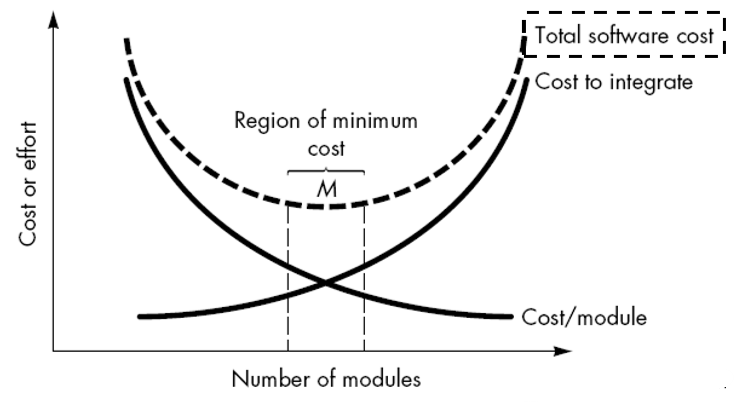
\includegraphics[width=.7\textwidth]{Immagini/decomposizionegraph.png}
\end{center}
Quindi dal grafico sappiamo che non si deve dividere troppo nè troppo poco.
\subsubsection{Modularità}
\customfbox{\textbf{Modulo}: è un'entità SW, identificata da un nome che può fornire servizi software; contiene istruzioni, strutture dati, controllo; può essere incluso in un altro modulo; può usare un altro modulo o parte di esso con la relazione 'dipende da'}
E' una conseguenza del principio di decomposizione, l'idea è quella di tenere separati gli aspetti "unrelated" di un software (\textbf{Separation of concerns}). Una valida linea guida è tenere separati il SW di generazione dati dal SW necessario alla loro presentazione e permette di cambiare la rappresentazione sullo schermo senza dover modificare il sistema di calcolo. La struttura di un'applicazione software, è spesso caratterizzata da tre livelli:
\begin{itemize}
    \item \textbf{Presentazione}: insieme dei moduli che gestiscono l'interazione con l'utente
    \item \textbf{Logica Applicativa}: insieme dei moduli che realizzano la logica applicativa, implementano le funzionalità richieste e gestiscono il flusso dei dati
    \item \textbf{Dati e Risorse}: insieme dei moduli che gestiscono i dati che rappresentano le informazioni utilizzate
\end{itemize}
Per modularizzare sostanzialmente bisogna fare in modo che ogni modulo esegua un singolo compito e minimizzare il numero e la complessità delle interconnessioni fra moduli. Dei moduli coesi e poco accoppiati sono\begin{itemize}
    \item facili da comprendere
    \item riusabili
    \item semplici da modificare
    \item semplici da testare
\end{itemize}
Bisogna evitare i moduli "monster" e per far ciò bisogna seguire i criteri per una buona modularizzazione: moduli piccoli, separation of concerns, alta coesione e basso accoppiamento e usare delle metriche o delle view per vedere se i criteri sono stati applicati.\\
Un modulo \textbf{coeso} svolge un \underline{unico compito}, in altre parole coesione è quando un modulo deve esprimere una sola astrazione, esistono diverse tipologie di coesione ma di solito si intende quella \textbf{funzionale}: tutti gli elementi del modulo contribuiscono ad un singolo ben definito task.\\
\customfbox{Ogni modulo non deve dipendere da troppi altri moduli, nè dipendervi in modo troppo forte}
Il coupling misura (informalmente) il grado di dipendenza di un modulo dagli altri e come prima non bisogna collegarli troppo e troppo poco.
\begin{itemize}
    \item Accoppiamento buono: chiamata di routine/metodo/funzione di altro modulo, uso di tipo di dato definito in altro modulo, inclusione o importazione di un package o di una libreria
    \item Accoppiamento cattivo: content coupling, un modulo modifica il valore di una variabile in un altro modulo
\end{itemize}
L'accoppiamento cattivo va evitato perchè complica enormemente la compresione e la modifica, in un sistema OO si riduce incapsulando tutti i campi di una classe dichiarandoli privati e fornendo i metodi di get e set. Nei linguaggi 'Legacy' le cose sono più complicate\ldots
\begin{itemize}
    \item \textbf{Fan-in}: numero di archi entranti in un modulo
    \item \textbf{Fan-out}: numero degli archi uscenti da un modulo
\end{itemize}
Un alto numero di Fan-in indica un buon riuso, un alto numero di Fan-out indica eccessiva dipendenza e che il modulo "fa troppo" (va decomposto).\\
\textbf{Generalità}: è la proprietà di design che "migliora" il riuso di un modulo in altri progetti (in futuro), si cerca di rendere un modulo il più generale possibile in modo da poterlo usare in più contesti. Questo principio è controverso perchè 'peggiora' un altro principio quello della 'semplicità' (KISS).
\subsection{Principio KISS}
Il design dovrebbe essere il più semplice possibile.
\begin{itemize}
    \item Keep It Simple, Stupid
    \item Keep It Short and Simple
\end{itemize}
\subsection{Sto seguendo i principi?}
Esistono delle metriche del SW che ci permettono di misurare l'aderenza a principi che abbiamo visto:
\begin{itemize}
    \item Metrica SW, ovvero la misura quantitativa del grado di possesso di uno specifico attributoda parte di un sistema, un componente, o un processo (es. LCOM (Lack of Cohesion))
    \item Esistono dei tool che forniscono  metriche e viste
\end{itemize}
\textbf{Esempio di metrica LCOM}
\begin{center}
    LCOM = numero di intersezioni vuote - numero di intersezioni non vuote
\end{center}
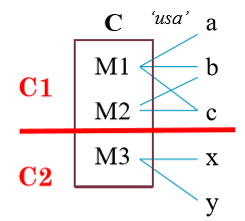
\includegraphics[width=0.3\textwidth]{Immagini/esempioLCOM.png}
Le intersezioni saranno $I_{1}=\{a,b,c\},I_{2}=\{b,c\},I_{3}=\{x,y\}$ quindi si avrà che $I_{1}\cap I_{2} \neq \emptyset $ mentre $I_{1}\cap I_{3} =I_{2}\cap I_{3} = \emptyset$ quindi avremo che $LCOM = 2-1 = 1$ e visto che è $>0$ classe $C$ non è coesa.
\chapter{UML - Introduzione}
\section{Cos'è}
L'UML è una famiglia di notazioni grafiche utili a supportare la descrizione e il progetto dei sistemi software. E' stato proposto come standard dall'OMG (Object Management Group) che ha come obiettivo di creare standard nel contesto IT.\\
E' unificato perchè in pratica è una collezione di varie notazioni preesistenti (Rumbaugh, Booch, Jacbson, Harel), integrate e rese Object Oriented.\\
L'UML \textbf{non} è:
\begin{itemize}
    \item Un metodo/processo di sviluppo $\rightarrow$ e' un linguaggio/notazione
    \item Un linguaggio di programmazione $\rightarrow$ è un linguaggio di modellazione
    \item Legato a UP (Unified Process) $\rightarrow$ è indipendente dal processo
\end{itemize}
L'UML può essere usato in diversi modi: 
\begin{itemize}
    \item \textbf{Abbozzo (sketch)}: per aiutare la comunicazione e la discussione
    \item \textbf{Progetto dettagliato (blueprint)}: per fornire un modello completo/dettagliato da implementare
    \item \textbf{Linguaggio di programmazione}: per fornire un "modello eseguibile"
\end{itemize}
\section{Prospettive}
\begin{itemize}
    \item \textbf{Prospettiva software}: gli elementi rappresentati sono elementi di un sistema software, serve per descrivere il design di un sistema software e per documentare un sistema software
    \item \textbf{Prospettiva concettuale}: gli elementi rappresentati sono concetti del dominio e serve per modellare il dominio del business e i processi
\end{itemize}
\section{Modello di dominio (del business)}
E' una rappresentazione visuale di classi concettuali o di oggetti del mondo reale di un dominio ed è un glossario visuale delle astrazioni significative del dominio.\\
E' utile per:
\begin{itemize}
    \item Chiarire i concetti di dominio nel quale il sistema software che dobbiamo progettare andrà inserito
    \item Ispirare nomi di alcune classi e attributi software nel design
    \item La progettazione del sistema
\end{itemize}
\section{Un po' di storia}
\begin{center}
    \begin{tikzpicture}
        % draw a horizontal line
        \draw (0,0) -- (18.5,0);
        
        % draw vertical lines
        \foreach \x in {1,3.5,5.5,7.5,9.5,11.5,13.5,15.5,17.5}
        \draw (\x cm,3pt) -- (\x cm,-3pt);
        
        % draw nodes to add events
        \draw (1,0) node[above=3pt] {Anni '80} node[below=3pt] {
        \begin{varwidth}{2cm}
            \begin{center}
                \footnotesize
                Linguaggi ad oggetti iniziano a prendere piede
            \end{center}
        \end{varwidth}
        };
        \draw (3.5,0) node[above=3pt] {1980-1995} node[below=3pt] {
            \begin{varwidth}{2cm}
                \begin{center}
                    \footnotesize
                    "babele" di linguaggi di modellazione
                \end{center}
            \end{varwidth}
        };
        \draw (5.5,0) node[above=3pt] {1994} node[below=3pt] {
            \begin{varwidth}{2cm}
                \begin{center}
                    \footnotesize
                    Rumbaugh si unisce a Booch alla Rational Software (azienda)
                \end{center}
            \end{varwidth}
        };
        \draw (7.5,0) node[above=3pt] {1995} node[below=3pt] {
            \begin{varwidth}{2cm}
                \begin{center}
                    \footnotesize
                    Booch e Rumbaugh presentano OOPSLA Unified Method v 0.8 \\
                    Viene dato l'annuncio che Ratinal ha comprato Objctory dove lavora Jacobson
                \end{center}
            \end{varwidth}
        };
        \draw (9.5,0) node[above=3pt] {1996} node[below=3pt] {
            \begin{varwidth}{2cm}
                \begin{center}
                    \footnotesize
                    OMG entra in campo sollecitata dai venditori di strumenti software terrorizzati dalla possibilità che Rational creasse un standard de-facto
                \end{center}
            \end{varwidth}
        };
        \draw (11.5,0) node[above=3pt] {1997} node[below=3pt] {
            \begin{varwidth}{2cm}
                \begin{center}
                    \footnotesize
                    call for proposal da parte di OMG. \\
                    "Tre amigos" presentano UML 1.0
                \end{center}
            \end{varwidth}
        };
        \draw (13.5,0) node[above=3pt] {11/1997} node[below=3pt] {
            \begin{varwidth}{2cm}
                \begin{center}
                    \footnotesize
                    Nasce UML 1.1 (standard OMG)
                \end{center}
            \end{varwidth}
        };
        \draw (15.5,0) node[above=3pt] {03/2005} node[below=3pt] {
            \begin{varwidth}{2cm}
                \begin{center}
                    \footnotesize
                    UML 2.0 diventa la versione ufficiale
                \end{center}
            \end{varwidth}
        };
        \draw (17.5,0) node[above=3pt] {Adesso} node[below=3pt] {
            \begin{varwidth}{2cm}
                \begin{center}
                    \footnotesize
                    UML 2.5.1
                \end{center}
            \end{varwidth}
        };
    \end{tikzpicture}
\end{center}
\section{Perchè}
Studiare UML è utile perchè è uno standard, è usato/richiesto dall'industria (almeno a livello di abbozzo) ed è indispenabile per le figure di Analista e Progettista (architetto) software.\\
Non lo studieremo in modo approfondito perchè, ad esempio, l'approccio blueprint è  poco usato nell'industria.
\section{Notazione e meta-modello}
UML definisce una famiglia di notazioni e un meta-modello.
\customfbox{Notazione = sintassi grafica del linguaggio \\ Meta-modello = definisce i concetti stessi del linguaggio}
\textbf{Esempio di meta-modello}: UML di una classe (generica) Java
\begin{center}
    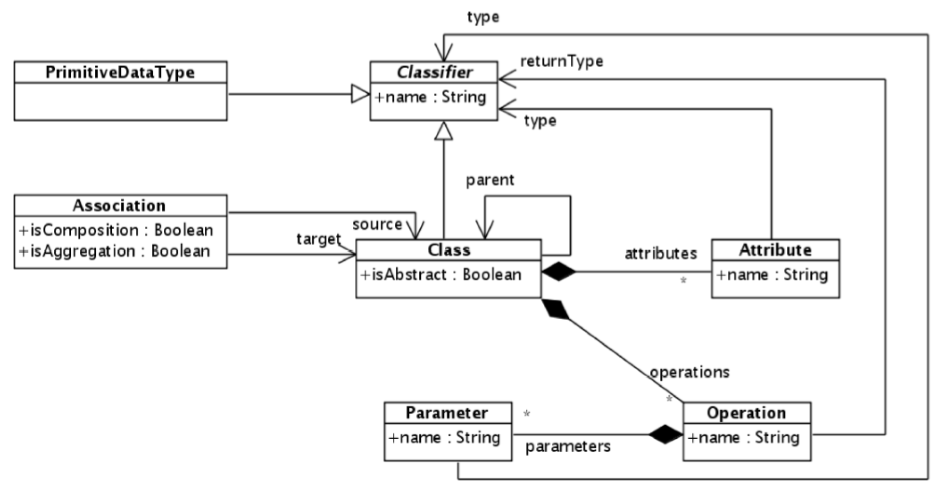
\includegraphics[width=.8\textwidth]{Immagini/UMLmetamodello.png}
\end{center}
In UML un sistema viene descritto utilizzando diverse viste e diversi diagrammi
\customfbox{Vista = particolare aspetto di un sistema SW dal punti di vista di uno specifico ruolo}
Un diagramma descrive/presenta una view/subview, chiameremo \textbf{Modello} un insieme di diagrammi che descrivono aspetti diversi dello stesso sistema SW. In un modello bisogna fare attenzione a non avere viste possibilmente sovrapposte (problema di consistenza) e incomplete (problema di completezza).\\
Il diagramma UML non è abbastanza e per questo esistono due soluzioni:
\begin{itemize}
    \item Si cerca o si produce un "estensione" di UML (profilo UML)
    \item Si usano diagrammi non UML
\end{itemize}
Facendo ciò si perde uno dei  vantaggi di UML: la standardizzazione.
\subsection{Profilo}
Come anticipato, UML si può estendere tramite il concetto di profilo per avere la possibilità di specificare particolari domini applicativi o tipologie di applicazioni.\\
Un profilo è costituito principalmente da:
\begin{itemize}
    \item \textbf{Stereotipi}: elementi aggiuntivi ottenuti modificando quelli esistenti
    \item \textbf{Vincoli aggiuntivi}
    \item \textbf{Informazioni semantiche aggiuntive} relative agli elementi aggiuntivi
\end{itemize}
\customfbox{Non si può guardare un diagramama UML e dire esattamente cosa farà il codice corrispondente}
Esiste un UML "legale"? La risposta è si e no: quello definito dalla specifica del  linguaggio (documento OMG) è quello legale ma UML è molto complesso e si presta a multiple interpretazioni, così le persone lo usano adottando convenzioni particolari (per semplificare) e quindi si perde la standardizzazione. Di solito si aggiunge nei diagrammi "\textbf{non-normativo}".
\section{Come usare UML}
\begin{enumerate}
    \item Capire il punti di vista dell''autore per capire i diagrammi
    \item Meglio dei buoni diagrammi "illegali" che altri formalmente corretti ma "scarsi"
    \item UML è molto complesso da prestarsi a multiple interpretazioni: usate un sottoinsieme e solo i diagrammi che ritenete utili (e che avete compreso bene)
    \item La completezza è nemica della chiarezza
    \item Qualsiasi informazione in UML può essere sempre soppressa
\end{enumerate}
\chapter{UML - Class Diagram}
\section{Introduzione}
Definisce:
\begin{itemize}
    \item Le classi
    \item Le loro feature \begin{itemize}
        \item Attributi
        \item Operazioni
    \end{itemize}
    \item Le relazioni tra classi \begin{itemize}
        \item Associazioni
        \item Aggregazione/Composizione
        \item Specializzazione/Generalizzazione
        \item Dipendenze
    \end{itemize}
\end{itemize}
Ovvero la parte statica di quello che intendiamo modellare.
\section{Prospettive}
Il significato di un class diagram e dei suoi elementi dipende dalla prospettiva:
\begin{itemize}
    \item Prospettiva concettuale: descriviamo gli elementi del "pezzo di mondo" che ci interessa modellare, la classe UML è un concetto proprio del dominio e un'operazione UML è un'azione/responsabilità
    \item Prospettiva software: descriviamo il design di un software, ovvero i modulo software che costituiranno l'implementazione vera e propria del sistema, la classe UML è una classe in un linguaggio OO e un'operazione UML è implementata da un metodo
\end{itemize}
\section{Classe}
Il concetto di classe è lo stesso dell'OO, incapsula caratteristiche comuni ad un gruppo di progetti, una classe genera oggeto con \texttt{create()} e un oggetto è un istanza di una classe. Gli attributi determinano lo stato degli oggetti mentre le operazioni descrivono il comportamento. Gli oggetti connessi tra loro possono collaborare per compiere task più complessi mediante scambio di messaggi.
\subsection{Rappresentazione}
Una classe in UML è semplicemente rappresentata da un rettangolo con il nome della classe all'interno, possiamo aggiungere gli attributi e le operazioni.
\begin{center}
    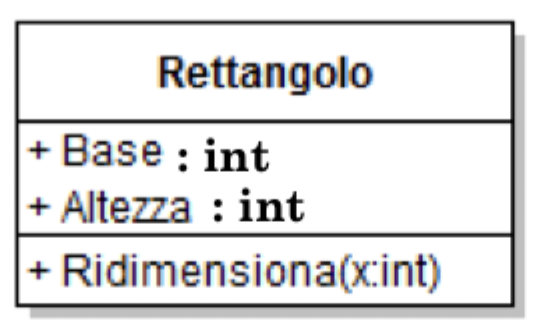
\includegraphics[width=.3\textwidth]{Immagini/UMLClass.png}
\end{center}
Se una classe è \texttt{abstract} viene indicata con il nome in corsivo.\\
Si ha una dipendenza tra due classi se la modifica di una classe può avere effetto sull'altra, si rappresenta con una freccia tratteggiata.
\subsection{Attributi}
\begin{center}
    \texttt{visibilità nome: tipo [molteplicità] = default \{proprietà\}}
\end{center}
\begin{itemize}
    \item \textbf{Visibilità}: \begin{itemize}
        \item \texttt{+}: pubblico
        \item \texttt{-}: privato
        \item \texttt{\#}: protetto
        \item \texttt{\~}: package
    \end{itemize}
    \item Il nome dell'attributo è l'unica parte obbligatoria
    \item Il tipo dell'attributo può essere: \begin{itemize}
        \item Primitivo
        \item Il nome di una classe definita nello stesso modello
    \end{itemize}
    \item Default rappresenta il valore di default dell'attributo di un oggetto appena creato
    \item Proprietà aggiuntive (es. \texttt{readOnly})
\end{itemize}
Le regole di visibilità tra i vari linguaggi e UML sono spesso differenti.\\
Gli attributi possono essere \texttt{static} e, come per il linguaggio Java, gli oggetti di una stessa classe condividono lo stesso valore per un attributo. In UML si indica sottolineando il nome dell'attributo.
\subsection{Molteplicità}
La molteplicità indica il quntitativo degli attributi, alcuni valori possibili sono:
\begin{itemize}
    \item 1 (uno e uno solo). E' il valore di default
    \item 0..1 (al più uno)
    \item * (un numero imprecisato, eventualmente nessuno)
    \item 1..* (almeno uno)
    \item n..m con $m\geq 1$
\end{itemize}
Gli elementi di un attributo con molteplicità $>1$ sono considerati come un insieme, se essi sono dotati anche di ordine si aggiunge la proprietà \texttt{\{ordered\}}
\subsection{Operazioni}
\begin{center}
    \texttt{visibilità nome (lista parametri) : tipo-ritornato {proprietà}}
\end{center}
\begin{itemize}
    \item Visibilità e nome stesse regole degli attributi
    \item Lista parametri contiene nome e tipo dei parametri, secondo la forma \texttt{direzione nome : tipo = default}
    \item Direzione: input (in), output (out) o entrambi (inout). Il valore di default è in.
    \item nome, tipo e valore di default sono analoghi a quelli degli attributi
    \item Tipo-ritornato è il tipo del valore di ritorno
\end{itemize}
\customfbox{Le operazioni get/set di solito non si indicano perchè è scontato che esistono}
In UML esistono due tipi di operazioni:
\begin{itemize}
    \item \textbf{Query} che ottengono un valore da un oggetto senza side efficiente
    \item \textbf{Modificatori} che modificano gli attributi (lo stato) dell'oggetto su cui sono chiamate
\end{itemize}
Un operazione può essere \texttt{static} e, come per il linguaggio Java, le operazioni non operano solo su una particolare istanza della classe ma sulla classe stessa. in UML si indica sottolineando il nome dell'operazione.
\customfbox{Un operazione viene invocata su un oggetto e corrisponde alla dichiarazione di una procedura/funzione, un metodo è il corpo di tale procedura/funzione, è l'implementazione di un operazione}
Se un'operazione è \texttt{abstract} viene indicata con il nome in corsivo.
\section{Datatype}
In UML esiste il concetto di datatype, per sua natura un oggetto ha un identità mentre un datatype no: le istanze sono valori non oggetti. Si rappresentano come classi con lo stereotipo \texttt{<<datatype>>}
\section{Associazioni}
\customfbox{Un'associazione rappresenta una relazione tra classi}
Il \texttt{>} indica in che direzione deve essere letta l'associazione, in alternativa si può indicare il ruolo di uno dei due estremi dell'associazione. In un diagramma delle classi non è consigliato aggiungere nomi delle associazioni e ruoli. \\
Il verso di navigazione indica in quale direzione è possibile reperire le informazioni ($\rightarrow$).
\subsection{Molteplicità}
La molteplicità delle associazioni indica il numero di link tra gli oggetti delle classi e, come in SQL, si mettono sulla freccia ai due estremi.
\subsection{Attributi}
Di solito si usano attributi per tipi primitivi e datatype o associazioni se tipati da classi.\\
Un associazione riflessiva è quando una classe ha un'associazione con se stessa.
\subsection{Implementazione (Java)}
\begin{itemize}
    \item Associazione molteplicità 1: \texttt{attributo}
    \item Associazione molteplicità 0..*: \texttt{HashSet}
    \item Associazione molteplicità \{ordered\} 0..*: \texttt{LinkedList} o \texttt{ArrayList}
\end{itemize}
Esistono anche le associazioni bidirezionali ma non possono essere implementate con un singolo attributo. Con le associazioni bidirezionali 1..1 c'è un problema di sincronizzazione.
\section{Note}
E' un commento in un linguaggio di programmazione, si usa anche per specificare il "behaviour" di un'operazione
\section{Aggregazione}
Rappresenta la relazione "tutto-parti", è una relazione di tipo "è composto da" e si rappresenta con un rombo vuoto.
\section{Composizione}
\textbf{Forma forte} di aggregazione: esprime la relazione "ha-un"/"è composto di", le proprietà sono:
\begin{itemize}
    \item Se il composto/intero viene distrutto, anche le sue parti saranno distrutte
    \item Una parte può appartenere ad un solo oggetto intero alla volta
\end{itemize}
\begin{itemize}
    \item \textbf{Generalizzazione = relazione "è un"}, ogni istanza di una classe è anche istanza della superclasse
    \item \textbf{Ereditarietà}: meccanismo attraverso il quale elementi specializzati incorporano la struttura ed il comportamento di elementi più generali. Nella classe erede è possibile aggiungere nuovi attributi e operazioni e ridefinire le operazioni (overriding)
\end{itemize}
\section{Generalizzazione ed ereditarietà}
\chapter{UML - Sequence Diagram}
\chapter{UML - State Machine \& Activity Diagram}
\chapter{UML - Component, Package \& Deployment Diagram}
\end{document}